\documentclass[../main.tex]{subfiles}
\usepackage[compat=1.1.0]{tikz-feynman}
\graphicspath{{../images/}}

\begin{document}
\hrule
\section{Quantum Electrodynamics}
\hrule \vspace{10px}

\lhead{Lecture 19: 4/1/24}
\chead{Quantum Electrodynamics}
\rhead{PHYS 474}

\paragraph*{Quiz Review} 
\paragraph*{Schrodinger Equation}
\begin{align*}
    E = \frac{\vb p^2}{2m} + v \to \qt(i\hbar \pdv{t})\psi = \qt(-\frac{\hbar^2}{2m} \laplacian + v) \psi
\end{align*}
where we apply
\begin{align*}
    \vb p \to -i\hbar \grad \\
    E \to i\hbar \pdv{t}
\end{align*}
and
\begin{align*}
    p_\mu \to i\hbar \partial_\mu \\
    p_0 = \frac{E}{c} \to i\hbar \pdv{t} \\
\end{align*}
\paragraph*{Relativistic Equation}
\begin{align*}
    E^2 = \vb p^2 c^2 + m^2 c^4
\end{align*}
so
\begin{align*}
    p_\mu p^\mu &= m^2 c^2 \\
    [(i\hbar \partial^\mu) (i\hbar \partial_\mu)] \psi &= m^2 c^2 \psi \\
    \implies (-\hbar^2 \partial^\mu \partial_\mu) \psi &= m^2 c^2 \psi \\
    \implies -\partial^\mu \partial_\mu \psi &= \frac{m^2 c^2}{\hbar^2} \psi \\
    \implies - \boxed{} \psi = \frac{m^2 c^2}{\hbar^2} \psi
\end{align*}
Which is the \emph{Klein-Gordan} equation where the box operator is the d'Alembertian operator. This
only describes spin-0 particles as a 2nd order in time derivative.

\paragraph*{Dirac Equation} To describe spin-1/2 particles, we need a relativistic wave eqn in the
1st order in time. Setting $\vb p = 0$ or at rest,
\begin{align*}
    \partial^\mu \partial_\mu \to \partial^0 \partial_0 = \pdv[2]{t} \\
    p_\mu = (p_0, \vb 0) \\
    p^\mu p_\mu = m^2 c^2 \\
    \qor p^0 p_0 = m^2 c^2 \qqtext{if} \vb p = 0 \\
    \qor p_0^2 - m^2 c^2 = 0 \\ 
    \qor (p^0 + mc) (p^0 - mc) = 0 \\
    \qor p^0 = \pm mc \\
    \qor i\hbar \pdv{t} \psi = \pm mc \psi 
\end{align*}
which gives us the Plane wave solution
\begin{align*}
    \psi(t) = \psi(0) e^{\pm i \frac{mc^2}{\hbar} t}
\end{align*}
If $\vb p \neq 0$, then from the dirac equation
\begin{align*}
    p^\mu p_\mu - m^2 c^2 = 0
\end{align*}
and writing into the form
\begin{align*}
    (\beta_K p^K + mc)(\gamma^\lambda p_\lambda - mc) = 0
\end{align*}
expanding out the terms
\begin{align*}
    \beta_K \gamma^\lambda p^K p_\lambda - mc(\beta_K p^K - \gamma^\lambda p_lambda) - m^2 c^2 = 0
\end{align*}
and since we are using dummy indices:
\begin{align*}
    \gamma^\lambda p_\lambda = \gamma_\lambda p^\lambda = \gamma_k p^K
\end{align*}
or
\begin{align*}
    \beta_K \gamma^\lambda p^K p_\lambda - mc(\beta_K- \gamma_k)p^K - m^2 c^2 = 0
\end{align*}
and comparing with
\begin{align*}
    p^\mu p_\mu - m^2 c^2 = 0
\end{align*}
which implies that the linear term in $p^\mu$ must be zero
\begin{align*}
    \implies \beta_K = \gamma_K
\end{align*}
so the equation becomes
\begin{align*}
    \gamma_K \gamma^\lambda p^K p_\lambda - m^2 c^2 = 0
\end{align*}
So we have the terms
\begin{align*}
    \implies \gamma_0 \gamma^0 p^0 p^0 + \gamma_1 \gamma^1 p^1 p_1 
    + \gamma_2 \gamma^2 p^2 p_2 + \gamma_3 \gamma^3 p^3 p^3  \\
    + \gamma_0 \gamma^1 p^0 p_1 + \dots - m^2 c^2 = 0
\end{align*}
The LHS should be equal to
\begin{align*}
    p^0 p_0 + p^1 p_1 + p^2 p_2 + p^3 p_3 - m^2 c^2 = 0
\end{align*}
so
\begin{align*}
    \gamma_0 \gamma^0 = \gamma_1 \gamma^1 = \gamma_2 \gamma^2 = \gamma_3 \gamma^3 = 1
\end{align*}
and the cross terms should be zero
\begin{align*}
    \gamma_0 \gamma^1 = \gamma_1 \gamma^0 = \gamma_2 \gamma^3 = \gamma_3 \gamma^2 = 0   
\end{align*}
and
\begin{align*}
    \gamma_0 &= g_{0\mu} \gamma^\mu \\
        &= g_{00} \gamma^0 = \gamma^0 \\
    \gamma_1 &= g_{11} \gamma^1 = -\gamma^1 \\
\end{align*}
so 
\begin{align*}
    (\gamma^0)^2 = - (\gamma^j)^2 = 1 \quad (j = 1,2,3) \\
    \gamma^\mu \gamma^\nu = 0 \qqtext{if} \mu \neq \nu \\
    \{ \gamma^\mu, \gamma^\nu \} = 2g^{\mu\nu}
\end{align*}
We can try $\gamma^0 = 1$ and $\gamma^j = i$ but it does not satisfy the third anticommutator relation.
so $\gamma$s have to be matrices, or more specifcally a $4\times 4$ matrix (Dirac matrices). We 
obtain the Dirac equation we take out one of the terms
\begin{align*}
    (\gamma_K p^K + mc)(\gamma^\lambda p_\lambda - mc) = 0\\
    \implies \gamma_K p^K \pm mc = 0
\end{align*}
and from the relativistic relation
\begin{align*}
    p^K \to i\hbar \partial^K
\end{align*}
we get the Dirac equation
\begin{align*}
    (i\hbar \gamma^K \partial_K \pm mc) \psi = 0
\end{align*}
where we can interchange the indices, i.e.,
\begin{align*}
    \gamma^K \partial_K = \gamma^\lambda \partial_\lambda = \gamma_\mu \partial^\mu
\end{align*}
Since $\gamma^\mu$ is a $4\times 4$ matrix, we have a Dirac spinor
\begin{align*}
    \psi = \mqty(\psi_1 \\ \psi_2 \\ \psi_3 \\ \psi_4)
\end{align*}
Using the Dirac basis
\begin{align*}
    \gamma^0 = \mqty(I & 0 \\ 0 & -I) \quad \gamma^j = \mqty(0 & \sigma^j \\ -\sigma^j & 0)
\end{align*}
where the matrices are in spinor space and not in Lorentz space.
\paragraph*{Solution to the Dirac Equation} for
\begin{align*}
    (i\hbar \gamma^\mu \partial_\mu - mc) \psi = 0
\end{align*}
First consider the rest case $\vb p = 0$ so
\begin{align*}
    (i\hbar \gamma^0 \partial_0 - mc) \psi = 0 \\
    \implies \qt(i\hbar \gamma^0 \frac{1}{c} \pdv{t} - mc) \psi = 0 \\
    \implies \mqty(1 & 0 \\ 0 & -1) \dv{t} \psi =-\frac{imc^2}{\hbar} \psi
\end{align*}
and we write $psi$ as a two components
\begin{align*}
    \psi = \mqty(\psi_A \\ \psi_B), \quad \psi_A = \mqty(\psi_1 \\ \psi_2), \quad \psi_B = \mqty(\psi_3 \\ \psi_4)
\end{align*}
so
\begin{align*}
    \mqty(1 & 0 \\ 0 & -1) \mqty(\dv{t} \psi_A \\ \dv{t} \psi_B) = -\frac{imc^2}{\hbar} \mqty(\psi_A \\ \psi_B)
\end{align*}
which splits into two equations
\begin{align*}
    \dv{t} \psi_A = -\frac{imc^2}{\hbar} \psi_A \\
    \dv{t} \psi_B = \frac{imc^2}{\hbar} \psi_B
\end{align*}
so the solutions are
\begin{align*}
    \psi_A(t) = \psi_A(0) e^{-\frac{imc^2}{\hbar} t} \\
    \psi_B(t) = \psi_B(0) e^{\frac{imc^2}{\hbar} t}
\end{align*}
Which is similar to the plane wave solution in QM that has the factor
\begin{align*}
    \psi(t) = \psi(0) e^{- i \frac{E}{\hbar} t}
\end{align*}
but here the energy is $E = mc^2$. $psi_A$ is the particle solution and $psi_B$ is the antiparticle
solution. For the vectors
\begin{align*}
    \psi_A = \mqty(\psi_1 \\ \psi_2) \quad \psi_B = \mqty(\psi_3 \\ \psi_4)
\end{align*}
we have two basis vectors
\begin{align*}
    \mqty(1 \\ 0) \quad \mqty(0 \\ 1)
\end{align*}
so
\begin{align*}
    \psi_A(t) = e^{-imc^2 t/\hbar} \mqty(1 \\ 0 \\ 0 \\ 0), \quad e^{-imc^2 t/\hbar} \mqty(0 \\ 1 \\ 0 \\ 0)
\end{align*}
which corresponds to the electron spin up and spin down states. We also have
\begin{align*}
    \psi_B(t) = e^{imc^2 t/\hbar} \mqty(0 \\ 0 \\ 1 \\ 0), \quad e^{imc^2 t/\hbar} \mqty(0 \\ 0 \\ 0 \\ 1)
\end{align*}
For the positron spin up and spin down states respectively.
\paragraph*{General Case} $\vb p \neq 0$
\begin{align*}
    (i\hbar \gamma^\mu \partial_\mu - mc) \psi = 0
\end{align*}
We would expect a plane wave solution of the form
\begin{align*}
    \psi(x) = e^{-i p \cdot x/\hbar} \psi(0)
\end{align*}
or
\begin{align*}
    \psi = a e^{-i k \cdot x/\hbar} u(k)
\end{align*}
where $u(k)$ is the spinor part, and $a$ is the normalization constant. The derivative of the exponent 
will give 
\begin{align*}
    \partial_\mu \psi = - ik_\mu \psi 
\end{align*}
and back into the dirac equation
\begin{align*}
    (i\hbar \gamma^\mu (-i k_\mu) - mc) \psi = 0 \\
    \qor \qt(\gamma^\mu k_m - \frac{mc}{\hbar}) u = 0
\end{align*}
where we know that
\begin{align*}
    \gamma^0 = \mqty(I & 0 \\ 0 & -I) \quad \gamma^j = \mqty(0 & \sigma^j \\ -\sigma^j & 0)
\end{align*}
so using 
\begin{align*}
    \gamma^\mu k_\mu &= \gamma^0 k_0 - \gamma^j k^j \\
    &= \mqty(1 & 0 \\ 0 & -1) k_0 - \mqty(0 & \sigma^j \\ -\sigma^j & 0) k^j \\
    &= \mqty(k_0 1 & -\vb \sigma \cdot \vb k \\ \vb \sigma \cdot \vb k & -k_0 1)
\end{align*}
where we define a Weyl spinor
\begin{align*}
    u = \mqty(u_A \\ u_B) 
\end{align*}
So we get
\begin{align*}
    \mqty(k_0 - \frac{mc}{\hbar} & -\vb \sigma \cdot \vb k \\ \vb \sigma \cdot \vb k & -k_0 - \frac{mc}{\hbar}) \mqty(u_A \\ u_B) = 0
\end{align*}
which gives us the coupled equations
\begin{align*}
    (k_0 - \frac{mc}{\hbar}) u_A - \vb \sigma \cdot \vb k u_B = 0 \\
    \vb \sigma \cdot \vb k u_A - (k_0 + \frac{mc}{\hbar}) u_B = 0
\end{align*}
and we can solve this by solving for $u_A$ in the first equation and substituting into the second equation
\begin{align*}
    u_A = \frac{\vb \sigma \cdot \vb k}{k_0 - \frac{mc}{\hbar}} u_B
\end{align*}
and substituting the second eq to the first
\begin{align*}
    u_B &=  \frac{\sigma \cdot \vb k}{k_0 + \frac{mc}{\hbar}} u_A \\
    &= \frac{\sigma \cdot \vb k}{k_0 + \frac{mc}{\hbar}} \frac{\vb \sigma \cdot \vb k}{k_0 - \frac{mc}{\hbar}} u_B \\
    &= \frac{(\vb \sigma \cdot \vb k)^2}{(k^0)^2 - \qt(\frac{mc}{\hbar})2} u_A
\end{align*}
where
\begin{align*}
    (\vb \sigma \cdot \vb k)^2 = (k^0)^2 - \qt(\frac{mc}{\hbar})^2 \\
    \implies \vb k^2 = (k^0)^2 - \qt(\frac{mc}{\hbar})^2
\end{align*}
and from the relativistic relation
\begin{align*}
    k^2 = k^\mu k_\mu = (k^0)^2 - \vb k^2 = \qt(\frac{mc}{\hbar})^2
\end{align*}
this tells us that $\hbar k_\mu$ must be the momentum $p_\mu$

\newpage
\lhead{Lecture 20: 4/3/24}
\paragraph*{Quiz Review}
\begin{itemize}
    \item From the Dirac Spinor
    \begin{align*}
        \psi = \mqty(\psi_1 \\ \psi_2 \\ \psi_3 \\ \psi_4)
    \end{align*}
    we have the particles represented by the wavefunction $\psi_A$ and the antiparticles represented by
    the wavefunction $\psi_B$.
    \begin{align*}
        \psi_A = \mqty(\psi_1 \\ \psi_2) \quad \psi_B = \mqty(\psi_3 \\ \psi_4)
    \end{align*}
    \item Weyl Spinors describe either the particle or antiparticle
    \begin{align*}
        \psi = \mqty(u_A \\ u_B)
    \end{align*}
    When the particle is the same as the antiparticle, then the two spinors are related by 
    \begin{align*}
        u_A = i\sigma^2 u_B^*
    \end{align*}
    so the dirac spinor becomes
    \begin{align*}
        \psi = C \psi^*
    \end{align*}
    where $C$ is the charge conjugation (Majorana fermion).
    \item Dirac matrices must be atleast 4 dimensional. 
\end{itemize}
\paragraph*{Solutions to the Dirac equation}
\begin{align*}
    (i\hbar \gamma^\mu \partial_\mu - mc) \psi = 0
\end{align*}
General Solution
\begin{align*}
    \psi = a e^{-i k \cdot x} u(k)
\end{align*}
where $u(k)$ is the spinor part. Since
\begin{align*}
    k^2 = \qt(\frac{mc}{\hbar})^2 \implies (\hbar k)^2 = (mc)^2 = p^2 \\
    \implies \hbar k = \pm p \\
    \qor k_\mu = \pm \frac{p_\mu}{\hbar}
\end{align*}
where $+$ is the particle solution and $-$ is the antiparticle solution. The zeroth component would be
\begin{align*}
    k^0 = \pm \frac{p^0}{\hbar} = \pm \frac{E^0}{\hbar}
\end{align*}
so
\begin{align*}
    \psi &\propto e^{-i p \cdot x/\hbar} \\
    &= e^{\mp i p \cdot x/\hbar} \\
    &\to \begin{cases}
        e^{-i p \cdot x/\hbar} \psi_A \quad \text{Particle} \\
        e^{i p \cdot x/\hbar} \psi_B \quad \text{Antiparticle}
    \end{cases}
\end{align*}
From the solutions
\begin{align*}
    u_A = \frac{\vb \sigma \cdot \vb k}{k^0 - \frac{mc}{\hbar}} u_B \\
    u_B = \frac{\vb \sigma \cdot \vb k}{k^0 + \frac{mc}{\hbar}} u_A
\end{align*}
\paragraph*{Solution 1 $u^{(1)}$}
If we choose a solution $u_A = \mqty(1 \\ 0)$ (Choosing $u_A$ to be the particle solution), then
\begin{align*}
    u_B &= \frac{\vb \sigma \cdot \vb p/ \hbar}{p^0/\hbar + mc/\hbar} \mqty(1 \\ 0) \\
    &= \frac{\vb \sigma \cdot \vb p}{p^0 + mc} \mqty(1 \\ 0) \\
\end{align*}
and using
\begin{align*}
    \vb \sigma \cdot \vb p &= \sigma^1 p_x + \sigma^2 p_y + \sigma^3 p_z \\
    &= \mqty(0 & 1 \\ 1 & 0) p_x + \mqty(0 & -i \\ i & 0) p_y + \mqty(1 & 0 \\ 0 & -1) p_z \\
    &= \mqty(p_z & p_x - i p_y \\ p_x + i p_y & -p_z)
\end{align*}
we get 
\begin{align*}
    u_B = \mqty(p_z \\ p_x + ip_y) \frac{c}{E + mc^2}
\end{align*}
\paragraph*{Solution 2 $u^{(2)}$}
If we choose $u_A = \mqty(0 \\ 1)$, then
\begin{align*}
    u_B = \mqty(p_x - i p_y \\ -p_z) \frac{c}{E + mc^2}
\end{align*}
\paragraph*{Solution 3 $v^{(1)}$}
The third solution is to choose $u_B = \mqty(1 \\ 0)$, then (choosing the minus sign for $k$)
\begin{align*}
    u_A &= \frac{-\vb \sigma \cdot \vb p}{-p^0 - mc} \mqty(1 \\ 0) \\
    &= \frac{\vb \sigma \cdot \vb p}{p^0 + mc} \mqty(1 \\ 0) \\
    &= \mqty(p_z \\ p_x + i p_y) \frac{c}{E + mc^2}
\end{align*}
\paragraph*{Solution 4 $v^{(1)}$}
and similarly for $u_B = \mqty(0 \\ 1)$
\begin{align*}
    u_A = \mqty(p_x - i p_y \\ -p_z) \frac{c}{E + mc^2}
\end{align*}
So with the 4 solutions for $u(k)$ 
\begin{align*}
    u^{(1)} = N e^{-i p \cdot x \hbar} \mqty(1 \\ 0 \\ \frac{c}{E + mc^2} p_z \\ \frac{c}{E + mc^2} (p_x + i p_y)) \\
    u^{(2)} = N e^{-i p \cdot x \hbar} \mqty(0 \\ 1 \\ \frac{c}{E + mc^2} (p_x - i p_y) \\ -\frac{c}{E + mc^2} p_z) \\
    v^{(2)} = N e^{i p \cdot x \hbar} \mqty(\frac{c}{E + mc^2} p_z \\ \frac{c}{E + mc^2} (p_x + i p_y) \\ 1 \\ 0) \\
    v^{(1)} = N e^{i p \cdot x \hbar} \mqty(\frac{c}{E + mc^2} (p_x - i p_y) \\ -\frac{c}{E + mc^2} p_z \\ 0 \\ 1)
\end{align*}
where $u^{(1)}$ is the particle with spin up, $u^{(2)}$ is the particle with spin down, $v^{(1)}$ is the
antiparticle with spin down, and $v^{(2)}$ is the antiparticle with spin up.
So 
\begin{align*}
    \psi = \begin{cases}
        a e^{-i p \cdot x/\hbar} u^{(1)} \qor u^{(2)} \quad \text{Particle} \\
        a e^{i p \cdot x/\hbar} v^{(1)} \qor v^{(2)} \quad \text{Antiparticle}
    \end{cases}
\end{align*}
where $\psi^\dagger \psi = 1$ or 
\begin{align*}
    u^\dagger u = \frac{2E}{c} \qor v^\dagger v = \frac{2E}{c}
\end{align*}
\paragraph*{Nonrelativistic Limit} 
\begin{align*}
    \vb p = m \vb v, \quad E \approx mc^2
\end{align*}
so 
\begin{align*}
    \frac{c}{E + mc^2} p_z \approx \frac{c}{2mc^2} m v_z = \frac{v_z}{2c} \to 0
\end{align*}
and
\begin{align*}
    \frac{c}{E + mc^2} (p_x + i p_y) \approx \frac{v_x + i v_y}{2c} \to 0
\end{align*}
for $v \ll c$. 
\paragraph*{Dirac Equation in momentum space}
\begin{align*}
    (i\hbar \gamma^\mu \partial_\mu - mc) \psi &= 0 \\
    p_\mu \to i\hbar \partial_\mu \\
    (\gamma^\mu p_\mu - mc) u &= 0 \qqtext{Particle} \\
    (\gamma^\mu p_\mu + mc) v &= 0 \qqtext{Antiparticle}
\end{align*}
we usually use the notation $\cancel{p} = \gamma^\mu p_\mu$
\paragraph*{Spin Operator}
\begin{align*}
    \vb S = \frac{\hbar}{2} \vb*\Sigma = \frac{\hbar}{2} \mqty(\vb*\sigma & 0 \\ 0 & \vb*\sigma) \\
    S^2 = \frac{\hbar^2}{4} \mqty(\sigma^2 & 0 \\ 0 & \sigma^2)
\end{align*}
since $\sigma_i^2 = I$, $\sigma^2 = \sigma_x^2 + \sigma_y^2 + \sigma_z^2 = 3I$ so
\begin{align*}
    S^2 &= \frac{3\hbar^2}{4} I \\
    &= \frac{1}{2} \qt(\ohf + 1) \hbar^2 I \\
    &= S (S + 1) \hbar^2 I \\
    \implies & S = \ohf \hbar
\end{align*}
So for the total spin
\begin{align*}
    \vb J = \vb L + \vb S
\end{align*}
then 
\begin{align*}
    [H, \vb J] = 0
\end{align*}
from the Heisenberg equation of motion.
\begin{align*}
    \dv{0}{t} = i\hbar [H, 0] = 0
\end{align*}
We find that
\begin{align*}
    [H, \vb L] \neq 0 \\
    [H, \vb S] \neq 0
\end{align*}
or simply 
\begin{align*}
    [H, \vb L] = - [H, \vb S] 
\end{align*}
The Hamiltonion or total energy is
\begin{align*}
    H = c p^0 = c \sqrt{\vb p^2 c^2 + m^2 c^4}
\end{align*}
from the Dirac equation in momentum space, we know that
\begin{align*}
    \gamma^\mu p_\mu - mc = 0 \\
    \qor \gamma^0 p_0 + \gamma^j p_j - mc = 0 \\
    \qor \gamma^0 p_0 = -\gamma^j p_j + mc
\end{align*}
We know that
\begin{align*}
    \gamma^0 = \mqty(I & 0 \\ 0 & -I) \quad \gamma^j = \mqty(0 & \sigma^j \\ -\sigma^j & 0)
\end{align*}
squaring $\gamma^0$ gives the identity matrix so
\begin{align*}
    (\gamma^0)^2 p_0 &= - \gamma^0 \gamma^j p_j + mc \\
    p_0 &= - \gamma^0 \gamma^j p_j + mc \\
    &= \gamma^0 \gamma^j p^j - mc
\end{align*}
Thus
\begin{align*}
    H = c (\gamma^0 \vb*\gamma \cdot \vb p + mc)
\end{align*}
\paragraph*{Lorentz Transformation Properties}
Starting again from the Dirac Equation
\begin{align*}
    (i\hbar \gamma^v\partial_v - mc) \psi = 0
\end{align*}
Under Lorentz transformation we let
\begin{align*}
    \psi \to \psi' = S \psi \\
    (i\hbar \gamma^\mu \partial_\mu - mc) \psi' = 0
\end{align*}
We denote 
\begin{align*}
    \partial_\mu ' = \pdv{x^v}{x_\mu'} \partial{x^v} \equiv \pdv{x^v}{x_\mu'} \partial_v \\
    x^\mu \to^\Lambda x'^\mu
\end{align*}
We also have axioms for the Dirac matrices (they don't transform)
so 
\begin{align*}
    \qt(i\hbar \gamma^\mu \pdv{x^v}{x_\mu'} \partial_v - mc) S\psi' = 0
\end{align*}
Mutliplying by $S^{-1}$ on the left
\begin{align*}
    S^{-1} i\hbar \gamma^\mu\pdv{x^v}{x_\mu'} S (\partial_v  \psi) - mc \psi = 0
\end{align*}
so matching this to the original Dirac equation
\begin{align*}
    S^{-1} \gamma^\mu \pdv{x^v}{x_\mu'} S = \gamma^v
\end{align*}
Since the $S$ commutes we can write
\begin{align*}
    S^{-1} \gamma^\mu S \pdv{x^v}{x_\mu'} = \gamma^v
\end{align*}
If the frame moves along the $x$-axis, 
\begin{align*}
    \Lambda = \mqty(\gamma & -\beta \gamma & 0 & 0 \\ -\beta \gamma & \gamma & 0 & 0 \\ 0 & 0 & 1 & 0 \\ 0 & 0 & 0 & 1)
\end{align*}
where we have the lorentz factor 
\begin{align*}
    \gamma = \frac{1}{\sqrt{1 - \frac{v^2}{c^2}}}
\end{align*}
we can show that
\begin{align*}
    S = a_+ + a_- \gamma^0 \gamma^1 \qquad a_{\pm} = \pm \sqrt{\frac{1}{2} (\gamma \pm 1)}
\end{align*}
In matrix form 
\begin{align*}
    S = a_+ I + a_- \mqty(1 & 0 \\ 0 & -1) \mqty(0 & \sigma^1 \\ -\sigma^1 & 0)
\end{align*}
where $I$ is a 4x4 identity matrix and
\begin{align*}
    \sigma^1 = \mqty(0 & 1 \\ 1 & 0)
\end{align*}
\begin{align*}
    S = \mqty(a_+ & 0 & 0 & a_- \\ 0 & a_+ & a_- & 0 \\ 0 & -a_- & a_+ & 0 \\ a_- & 0 & 0 & a_+)
\end{align*}
a symmetric real matrix
\paragraph*{Invariant}
\begin{align*}
    \psi \to \abs{\psi}^2 = \psi^\dagger \psi = 1
\end{align*}
For invariant quantities in non relativistic QM. For relativistic transformations
\begin{align*}
    \psi^\dagger \psi \to^\Lambda (S \psi)^\dagger (S\psi) \\
    = \psi^\dagger S^\dagger S \psi \\
\end{align*}
But since $S$ is real and symmetric $S^\dagger = S$ So
\begin{align*}
    = \psi^\dagger S^2 \psi
\end{align*}
We find that
\begin{align*}
    S^2 = \gamma \mqty(I & -\frac{v}{c} \sigma_1 \\ -\frac{v}{c} \sigma_1 & I) \neq I
\end{align*}
So we need to find the lorentz invariant quanities (Bilinears)

\newpage
\lhead{Lecture 21: 4/10/24}
\paragraph*{Bilinears}
Under Lorentz transformations
\begin{align*}
    \psi^\dagger \psi \to \psi'^\dagger \psi' \\
    = (S\psi)^\dagger (S\psi) = \psi^\dagger S^\dagger S \psi
\end{align*}
Since $S$ is real and symmetric, $S^\dagger = S$ or $S^\dagger S = S^2$ where
\begin{align*}
    S^2 = \gamma \mqty(I & -\frac{v}{c} \sigma_1 \\ -\frac{v}{c} \sigma_1 & I) \neq I
\end{align*}
For $v \ll c, \quad S^2 \to I$. So we need to find a Lorentz invariant quantity, or the adjoint 
spinor, $\bar\psi = \psi^\dagger \gamma^0$:
\begin{align*}
    \bar\psi \psi \to \bar\psi' \psi' = (\psi'^\dagger \gamma^0) \psi' 
    = (S\psi)^\dagger \gamma^0 S \psi \\
    = \psi^\dagger S^\dagger \gamma^0 S \psi = \psi^\dagger \gamma^0 \psi = \bar \psi \psi
\end{align*}
This is one of the bilinears ($\bar \psi \psi$) that is lorentz invariant.
\paragraph*{Discrete Symmetry Operators}
\begin{align*}
    P &= \gamma^0 \qquad \psi(t, \vb x) \to \gamma^0 \psi(t, - \vb x) \\
    C &= i \gamma^2 \qquad \psi(t, \vb x) \to i \gamma^2 \psi^*(t, \vb x) \\
    T &= \gamma^1 \gamma^3 \qquad \psi(t, \vb x) \to \gamma^1 \gamma^3 \psi(-t, \vb x)
\end{align*}
So under parity
\begin{align*}
    \bar \psi \psi \to^P \bar\psi' \psi' &= \psi'^\dagger \gamma^0 \psi' \\
    &= (\gamma^0 \psi)^\dagger \gamma^0 (\gamma^0 \psi) \\
    &= \psi^\dagger \gamma^{0\dagger} (\gamma^0 \gamma^0) \psi \qquad \gamma^0 \gamma^0 = I \\
    &= (\psi^\dagger \gamma^0) \psi = \bar \psi \psi
\end{align*}
which is P-even. For The pseudoscalar
\begin{align*}
    \gamma^5 \equiv i \gamma^0 \gamma^1 \gamma^2 \gamma^3
\end{align*}
where
\begin{align*}
    \{\gamma^\mu, \gamma^v\} = 2g^{\mu v} \\
    \implies \{\gamma^\mu, \gamma^v\} = 0 \qqtext{if} \mu \neq v
\end{align*}
and
\begin{align*}
    \{\gamma^\mu, i \gamma^0 \gamma^1 \gamma^2 \gamma^3\} = i(\gamma^\mu \gamma^0 \gamma^1 \gamma^2 \gamma^3 + \gamma^0 \gamma^1 \gamma^2 \gamma^3 \gamma^\mu) \\
\end{align*}
And at $\mu = 0$:
\begin{align*}
    &= i (\gamma^0 \gamma^0 \gamma^1 \gamma^2 \gamma^3 + \gamma^0 \gamma^1 \gamma^2 \gamma^3 \gamma^0) \\
    &= i (\gamma^1 \gamma^2 \gamma^3 - \gamma^1 \gamma^2 \gamma^3) = 0 \qquad \gamma^\mu \gamma^v = - \gamma^v \gamma^\mu
\end{align*}
So
\begin{align*}
    \{\gamma^\mu, \gamma^5\} = 0
\end{align*}
So the Parity operator
\begin{align*}
    \bar\psi \gamma^5 \psi \to^P \bar\psi' \gamma^5 \psi' &= \psi'^\dagger \gamma^0 \gamma^5 \psi' \\
    &= (\gamma^0 \psi)^\dagger \gamma^0 \gamma^5 (\gamma^0 \psi) \\
    &= \psi^\dagger \gamma^{0\dagger} \gamma^0 \gamma^5 \gamma^0 \psi \\
    &= \psi^\dagger \gamma^5 \gamma^0 \psi = - \bar \psi \gamma^5 \psi
\end{align*}
which is P-odd. Thus the Bilinears are
\begin{enumerate}
    \item $\bar \psi \psi$: P-even (scalar)
    \item $\bar \psi \gamma^5 \psi$: P-odd (pseudoscalar)
    \item $\bar \psi \gamma^\mu \psi$: Vector
    \item $\bar \psi \gamma^\mu \gamma^5 \psi$: Axial Vector
    \item $\bar \psi \sigma^{\mu v} \psi$: Tensor where $\sigma^{\mu v} = \frac{i}{2} [\gamma^\mu, \gamma^v]$
\end{enumerate}
\paragraph*{Clifford Algebra}
Any $4\times 4$ matrix can be written in the basis of the five bilnears
\begin{align*}
    \{I, \gamma^5, \gamma^\mu, \gamma^\mu \gamma^5, \sigma^{\mu v}\}
\end{align*}
So there are
\begin{align*}
    1 + 1 + 4 + 4 + 6 = 16
\end{align*}
independent $4\times 4$ matrices.

\paragraph*{Momentum Space}
\begin{align*}
    (\gamma^\mu p_\mu - mc) u^{(s)} &= 0 \qqtext{(Particle)} \\
    (\gamma^\mu p_\mu + mc) v^{(s)} &= 0 \qqtext{(Antiparticle)} \\
    \bar u (\gamma^\mu p_\mu - mc) &= 0  \\
    \bar v (\gamma^\mu p_\mu + mc) &= 0
\end{align*}
where
\begin{align*}
    u^\dagger u = v^\dagger v = \frac{2E}{c} \\
    \implies \bar u u = - \bar v v = 2mc
\end{align*}
We also get the completeness relation
\begin{align*}
    \sum_{s = 1,2} u^{(s)} \bar u^{(s)} = \gamma^\mu p_\mu + mc \\
    \sum_{s = 1,2} v^{(s)} \bar v^{(s)} = \gamma^\mu p_\mu - mc
\end{align*}
In the basis states $\ket{a_i}$ where
\begin{align*}
    I = \sum_i \ket{a_i} \bra{a_i}
\end{align*}
so 
\begin{align*}
    \ket{\psi} = \sum_i \ket{a_i} \braket{a_i}{\psi} = \sum_i c_i \ket{a_i}
\end{align*}

\subsection*{Photon}
In QED we have just an electron/position and a photon. We found electron/positron but now to find
the photon. From the maxwell equations
\begin{align*}
    \div \vb E &= 4 \pi \rho \\
    \curl \vb E &= - \pdv{\vb B}{t} \\
    \div \vb B &= 0 \\
    \curl \vb B &= \frac{4\pi}{c} \vb J + \frac{1}{c} \pdv{\vb E}{t}
\end{align*}
THe EM field strength tensor $F^{\mu \nu}$ is defined as
\begin{align*}
    F^{\mu v} = \mqty(0 & -E_x & -E_y & -E_z \\ 
                        E_x & 0 & -B_z & B_y \\
                        E_y & B_z & 0 & -B_x \\
                        E_z & -B_y & B_x & 0)
\end{align*}
and the current vector $J^\mu = (\rho c, \vb J)$.
\paragraph*{Inhomogenous Maxwell Equations}
For the First and Fourth equations
\begin{align*}
    \partial_\mu F^{\mu \nu} = \frac{4\pi}{c} J^\nu
\end{align*}
where
\begin{align*}
    F^{\mu\nu} = - F^{\nu\mu}
\end{align*}
so
\begin{align*}
    \partial_\nu \partial_\mu F^{\mu\nu} = \frac{4\pi}{c} \partial_\nu J^\nu \\
    0 = \partial_\nu J^\nu
\end{align*}
Which is equivalent to the charge conservation
\begin{align*}
    \frac{1}{c}  \dv{\rho c}{t} + \div \vb J = 0 \\
    \dv{\rho}{t} + \div \vb J = 0 
\end{align*}
and integrating over a volume
\begin{align*}
    \int \dd{V} \qt(\dv{\rho}{t} + \div \vb J) = 0 \\
    \dv{t} \int \dd{V} \rho + \int \dd{V} \div \vb J = 0 
    \dv{Q}{t} + \oint \vb J \cdot \dd{\vb S} = 0
\end{align*}
From Gauss' Law so we do indead find that 
\begin{align*}
    \vb J = 0 \implies Q = \text{constant}
\end{align*}
From the Hemholtz potential we know that $\vb B = \curl \vb A$, so the second Maxwell eq is
\begin{align*}
    \curl \vb E =  - \frac{1}{c} \dv{t}(\curl \vb A)
\end{align*}
or
\begin{align*}
    \curl(\vb E + \frac{1}{c} \dv{\vb A}{t}) = 0
\end{align*}
or
\begin{align*}
    \vb E + \frac{1}{c} \dv{\vb A}{t} = - \grad V
\end{align*}
So we have an EM field
\begin{align*}
    A^\mu = (V, \vb A)
\end{align*}
where
\begin{align*}
    F^{\mu\nu} = \partial^\mu A^\nu - \partial^\nu A^\mu
\end{align*}
Which gives us the general Maxwell eq
\begin{align*}
    \partial_\mu (\partial^\mu A^\nu - \partial^\nu A^\mu) = \frac{4\pi}{c} J^\nu
\end{align*}
From the Gauge transformation
\begin{align*}
    A^\mu \to A'^\mu = A^\mu + \partial^\mu \lambda
\end{align*}
then 
\begin{align*}
    F^{\mu\nu} \to F'^{\mu\nu} = \partial^\mu A'^\nu - \partial^\nu A'^\mu \\
    = \partial^\mu (A^\nu + \partial^\nu \lambda) - \partial^\nu (A^\mu + \partial^\mu  \lambda) = F^{\mu\nu}
\end{align*}
THe Gauge fixing condition $\partial_\mu A^\mu = 0$ so the maxwell eq becomes
\begin{align*}
    \partial_\mu \partial^\nu A^\nu = \frac{4\pi}{c} J^\nu
\end{align*}
or
\begin{align*}
    \boxed{\;} A^\nu = \frac{4\pi}{c} J^\nu
\end{align*}
If $\boxed{\;} \lambda = 0$, choose a particular gauge, or the COulomb gauge
\begin{align*}
    A^0 = 0 
\end{align*}
in free space. For $\partial_\mu A^\mu = 0$
\begin{align*}
    \div \vb A = 0
\end{align*}
In free space there is no current density, $J^\mu = 0$
\begin{align*}
    \boxed{\;} A^\mu = 0
\end{align*}
which is the Klein-Gordan eq with mass $m = 0$. So the solution is a plane wave
\begin{align*}
    A^\mu = a e^{-ip x / \hbar} \epsilon^\mu
\end{align*}
where $\epsilon^\mu$ is the polarization vector. So
\begin{align*}
    \partial_\mu A^\mu = 0 \implies p_\mu \epsilon^\mu = 0
\end{align*}
and 
\begin{align*}
    \div{\vb A} = 0 \implies \vb p \cdot \vb*{\epsilon} = 0
\end{align*}
so $\vb*{\epsilon}$ is perpendicular to $\vb p$. The components of the vector are
\begin{align*}
    \vb p = p \vu z
\end{align*}
and 
\begin{align*}
    \epsilon^{(1)} = \mqty(1 \\ 0 \\ 0), \quad \epsilon^{(2)} = \mqty(0 \\ 1 \\ 0)
\end{align*}
so
\begin{align*}
    \epsilon_{\pm} = \frac{1}{\sqrt{2}} (\epsilon^{(1)} \pm i \epsilon^{(2)})
\end{align*}
or circular polarization. 
\paragraph*{Photon} 
We have
\begin{align*}
    A^\mu = a e^{-ip x/\hbar} \epsilon_{(s)}^\mu
\end{align*}
where $s = 1,2$ for two polarizations. The lorentz condition tells us $p_\mu \epsilon^\mu = 0$. And the
Coulomb gauge $\vb p \cdot \vb*\epsilon = 0$. The completeness relation
\begin{align*}
    \sum_{s = 1,2} \epsilon_i^{(s)} \epsilon_j^{(s_1)*} = \delta_{ij} - \vu p_i \vu p_j
\end{align*}

\newpage
\lhead{Lecture 22: 4/15/24}
\subsection*{Feynman Rules}
\begin{enumerate}
    \item \begin{itemize}
        \item External Momental: $p_i$
        \item Internal Momenta: $q_i$
    \end{itemize}
    \item \begin{itemize}
        \item Fermions: (straight line) Fermion and Momentum flow in same direction: $u^{(s)}(p)$ for incoming, 
        $\bar u^{(s)}(p)$ for outgoing
        % tikz feynman diagram of single fermion line
        \begin{center}
            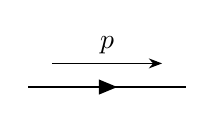
\begin{tikzpicture}
                \begin{feynman}
                    \vertex (a) at (0,0);
                    \vertex (b) at (2,0);
                    \diagram* {
                        (a) -- [fermion, momentum=$p$] (b);
                    };
                \end{feynman}
            \end{tikzpicture}
        \end{center}
        \item Anti-fermion: Fermion and Momentum flow in opposite direction: 
        $\bar v^{(s)}(p)$ for incoming, $v^{(s)}(p)$ for outgoing   
        % tikz feynman diagram of single anti-fermion line
        \begin{center}
            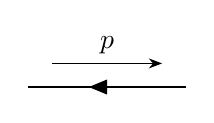
\begin{tikzpicture}
                \begin{feynman}
                    \vertex (a) at (0,0);
                    \vertex (b) at (2,0);
                    \diagram* {
                        (a) -- [anti fermion, momentum=$p$] (b);
                    };
                \end{feynman}
            \end{tikzpicture}
        \end{center}
        \item Photon: (wave line) $\epsilon_\mu (p)$ for incoming, $\epsilon_\mu^*(p)$ for outgoing
    \end{itemize}
    \item Vertex: $i g_e \gamma^\mu$ for fermion-photon vertex
    \begin{align*}
        g_e = \sqrt{4\pi \alpha} = \sqrt{4 \pi \frac{e^2}{\hbar c}} = e \sqrt{\frac{4\pi}{\hbar c}}
    \end{align*}
    \item Propogator: For the particle/antiparticle
    \begin{align*}
        \frac{i(\gamma^\mu q_\mu + mc)}{q^2 - m^2 c^2}
    \end{align*}
    For the photon
    \begin{align*}
        \frac{-i g_{\mu v}}{q^2}
    \end{align*}
    \item Conservation of four-momenta at each vertex
    \begin{align*}
        (2\pi)^4 \delta^4(k_1 + k_2 + k_3)
    \end{align*}
    where $k$'s are incoming momenta
    \item Integrate over internal momenta
    \begin{align*}
        \int \frac{\dd[4]{q_1}}{(2\pi)^4} \frac{\dd[4]{q_2}}{(2\pi)^4} \cdots
    \end{align*}
    \item Drop $(2\pi)^4 \delta^4(p_1 + p_2 + \dots - p_n - p_{n +1} - \dots)$
    \item Multiply the answer by $i$:
    \item Anti-symmetrization: Diagrams differing only by the inter change of identical fermions
    have a relative minus sign
\end{enumerate}

\paragraph*{Example:} $e$-$\mu$ scattering
% tikz feynman diagram of e-mu scattering
From the matrix multiplication we need $(1 \times 4) (4 \times 4) (4 \times 1)$ so
\begin{align*}
    \bar u(p_3) (ig_e \gamma^\mu) u(p_1)
\end{align*}
or in the opposite direction of the fermion flow. The amplitude is
\begin{align*}
    \mathcal{M} = i \int \frac{\dd[4]{q}}{(2\pi)^4} [\bar u^{(s_3)}(p_3) (ig_e \gamma^\mu) u^{(s_1)}(p_1)] 
    \qt(\frac{-ig_{\mu v}}{q^2}) [\bar u^{(s_4)}(p_4) (ig_e \gamma^\mu) u^{(s_2)}(p_2)] \\
    \times (2\pi)^4 \delta^4(p_1 - q - p_3) \delta^4(p_2 + q - p_4)
\end{align*}
and since $q = p_4 - p_2$ substituting in to the first delta function
\begin{align*}
    (2\pi)^4 \delta^4(p_1 - (p_4 - p_2) - p_4) = (2\pi)^4 \cancel{\delta^4(p_1 + p_2 - p_3 - p_4)}
\end{align*}
Which cancels out from rule 7. Thus we ge the amplitude
\begin{align*}
    \mathcal{M} = \frac{-g_e^2}{(p_4 - p_2)^2} [\bar u^{(s_3)}(p_3) \gamma^\mu u^{(s_1)}(p_1)]
     [\bar u^{(s_4)}(p_4) \gamma_\mu u^{(s_2)}(p_2)] \\
    g_{\mu v} \gamma^v = \gamma_\mu 
\end{align*}
Where
\begin{align*}
    p_1 + p_2 = p_3 + p_4 \\
    \implies p_4 - p_2 = p_1 - p_3
\end{align*}
and 
\begin{align*}
    \dv{\sigma}{\Omega} \propto \abs{\mathcal{M}}^2
\end{align*}

\paragraph*{Example:} $e^- e^-$ Scattering (M{\o}eller Scattering)
% tikz feynman diagram of e-e- scattering
If we have the diagram set horizontally, we actually have $e^- e^+ \to e^- e^+$ scattering 
(Bhabha Scattering). The first diagram is the same as the electron-muon scattering:
\begin{align*}
    \mathcal{M}_1 &= \frac{-g_e^2}{(p_1 - p_3)^2} [\bar u^{(s_3)}(p_3) \gamma^\mu u^{(s_1)}(p_1)]
     [\bar u^{(s_4)}(p_4) \gamma_\mu u^{(s_2)}(p_2)] \\
    \mathcal{M}_2 &= \frac{-g_e^2}{(p_1 - p_4)^2} [\bar u^{(s_4)}(p_4) \gamma^\mu u^{(s_2)}(p_2)]
     [\bar u^{(s_3)}(p_3) \gamma_\mu u^{(s_1)}(p_1)]
\end{align*}
since the momentum of $p_3$ and $p_4$ are interchanged so the total amplitude is
\begin{align*}
    \mathcal{M} = \mathcal{M}_1 - \mathcal{M}_2
\end{align*}
where the minus sign comes from rule 9, or the interchange of identical fermions.

\paragraph*{Example:} $e^- e^+$ Scattering (Bhabha Scattering)
The bottom part of the diagram is the same as the electron-muon scattering:
\begin{align*}
    \mathcal{M}_1 = i \int \frac{\dd[4]{q}}{(2\pi)^4} [\bar u^{(s_3)}(p_3) (ig_e \gamma^\mu) u^{(s_1)}(p_1)] \\
    \times \qt(\frac{-i g_{\mu v}}{q^2}) [\bar v^{(s_2)}(p_2) (ig_e \gamma^\mu) v^{(s_4)}(p_4)] \\
    \times (2\pi)^4 \delta^4(p_1 - q - p_3) \delta^4(p_2 + q - p_4)
\end{align*}
and again using $q = p_4 - p_2$ we can cancel out the delta functions
\begin{align*}
    = -\frac{g_e^2}{(p_4 - p_2)^2} [\bar u^{(s_3)}(p_3) \gamma^\mu u^{(s_1)}(p_1)]
    [\bar v^{(s_2)}(p_2) \gamma_\mu v^{(s_4)}(p_4)]
\end{align*}
for the first diagram, and the second diagram is a combination:
\begin{align*}
    \mathcal{M}_2 = i \int \frac{\dd[4]{q}}{(2\pi)^4} [\bar v^{(s_2)}(p_2) (ig_e \gamma^\mu) u^{(s_1)}(p_1)] \\
    \times \qt(\frac{-i g_{\mu v}}{q^2}) [\bar u^{(s_3)}(p_3) (ig_e \gamma^\mu) v^{(s_4)}(p_4)] \\
    \times (2\pi)^4 \delta^4(p_1 + p_2 - q) \delta^4(q - p_3 - p_4)
\end{align*} 
using the second delta function again $q = p_3 + p_4$ so
\begin{align*}
    p_1 + p_2 - q = p_1 + p_2 - p_3 - p_4
\end{align*}
so the amplitude is
\begin{align*}
    \mathcal{M}_2 = -\frac{g_e^2}{(p_3 + p_4)^2} [\bar v^{(s_2)}(p_2) \gamma^\mu u^{(s_1)}(p_1)]
    [\bar u^{(s_3)}(p_3) \gamma_\mu v^{(s_4)}(p_4)]
\end{align*}
and the total amplitude is
\begin{align*}
    \mathcal{M} = \mathcal{M}_1 - \mathcal{M}_2
\end{align*}
where the plus is because we have two different fermions\dots this is wrong. Interchanging the
2nd and 4th fermions on the second diagram gives the first diagram. 

\paragraph*{Matrix Elements}
\begin{align*}
    \dv{\sigma}{\Omega} = \qt(\frac{\hbar c}{8\pi})^2 \frac{S}{(E_1 + E_2)^2} \abs{\mathcal{M}}^2
    \frac{\abs{\vb p_f}}{\abs{\vb p_i}}
\end{align*}
so the squared factor 
\begin{align*}
    \abs{\mathcal{M}}^2 &= \frac{g_e^4}{(p_1 - p_3)^4} [\bar u^{(s_3)}(p_3) \gamma^\mu u^{(s_1)}(p_1)]
    [\bar u^{(s_4)}(p_4) \gamma_\mu u^{(s_2)}(p_2)] \\
    &\times [\bar u^{(s_3)}(p_3) \gamma^\nu u^{(s_1)}(p_1)]^\dagger
    [\bar u^{(s_4)}(p_4) \gamma_\nu u^{(s_2)}(p_2)]^\dagger
\end{align*}
where the Hermitian conjugate of the two terms are
\begin{align*}
    u^\dagger(p_1) \gamma^{\nu \dagger} \gamma^{0\dagger} u(p_3)
\end{align*}
multiplying by $\gamma^0 \gamma^0$:
\begin{align*}
    (u^\dagger(p_1) \gamma^0) \gamma^0 \gamma^{\nu \dagger} \gamma^{0\dagger} u(p_3) \\
    = \bar u(p_1) \gamma^0 \gamma^{\nu \dagger} \gamma^0 u(p_3) \\
    = \bar u(p_1) \gamma^\nu u(p_3)
\end{align*}
and similarly for the second term:
\begin{align*}
    \bar u(p_2) \gamma_\nu u(p_4)
\end{align*}
For the unpolarized cross sections we sum over the final spins and average over the initial spins:
\begin{align*}
    \abs{\mathcal{\bar M}}^2 = \frac{1}{4} \sum \sum
\end{align*}

\newpage
\lhead{Lecture 23: 4/17/24}
\paragraph*{Quiz Review:}
\begin{itemize}
    \item \begin{align*}
        \gamma^\mu \gamma_\mu &= \gamma^0 \gamma_0 + \gamma^1 \gamma_1 + \gamma^2 \gamma_2 + \gamma^3 \gamma_3 \\
        &= \gamma^0 g_{00} \gamma^0 + 3 \gamma^i \gamma^i g_{ii} \\
        &= 1 + 3 (-1)(-1) = 4
    \end{align*}
    \item Since $\cancel{a} \cancel{b} = a_\mu \gamma^\mu b_\nu \gamma^\nu$ we have
    \begin{align*}
        \Tr (\cancel{a} \cancel{b})  &= a_\mu b_\nu \Tr(\gamma^\mu \gamma^\nu)
    \end{align*}
    and since the Trace is cyclic
    \begin{align*}
        &= \frac{1}{2} a_\mu b_\nu \Tr(\gamma^\mu \gamma^\nu + \gamma^\nu \gamma^\mu) \\
        &= a_\mu b_\nu g^{\mu\nu} \Tr(I_{4x4}) = 4 a_\mu b^\mu = 4 a \cdot b
    \end{align*}
    \item $\gamma^5 = i \gamma^0 \gamma^1 \gamma^2 \gamma^3$ and from the cyclicity of the trace
    \begin{align*}
        \Tr (\gamma^\mu \gamma^5) &= \Tr(\gamma^5 \gamma^\mu) = -\Tr(\gamma^5 \gamma^\mu)
    \end{align*}
    which is only true if the trace is zero.
    \item From the anticommutator $\{\gamma^\mu, \gamma^\nu = 2 g^{\mu\nu} \}$ so
    \begin{align*}
        \Tr(\{\gamma^\mu, \gamma^\nu\}, \gamma^5) &= 2 g^{\mu\nu} \Tr(\gamma^5) = 0 \\
        &= \Tr(\gamma^\mu \gamma^\nu \gamma^5 + \gamma^\nu \gamma^\mu \gamma^5) = 0
    \end{align*}
    So the quantity is an antisymmetric tensor or rank 2, which does not exist. 
\end{itemize}
From the completeness relation
\begin{align*}
    \sum_{s = 1,2} u^{(s)} \bar u^{(s)} = \gamma^\mu p_\mu + mc = \cancel{p} + mc \\
    \sum_{s = 1,2} v^{(s)} \bar v^{(s)} = \cancel{p} - mc
\end{align*}
So from the squared amplitude:
\begin{align*}
    \abs{\mathcal{M}}^2 = \frac{g_e^4}{(p_1 - p_3)^4} [\bar u^{(s_3)}(p_3) \gamma^\mu u^{(s_1)}(p_1)]
    [\bar u^{(s_4)}(p_4) \gamma_\mu u^{(s_2)}(p_2)] \\
    \times [\bar u_1 \gamma^\nu u_3]
    [\bar u_2 \gamma_\nu u_4]
\end{align*}
we can rearrange the terms by writing the 3rd between the first and second terms and the 4th between the 2nd and 3rd terms:
\begin{align*}
    \sum_{s_1,s_2} \abs{\mathcal{M}}^2 = \frac{g_e^4}{(p_1 - p_3)^4} 
    [\bar u_3 \gamma^\mu (\sum_{s_1} u^{(s_1)}(p_1) \bar u^{(s_1)}(p_1)) \gamma^\nu u_3] \\
    [\bar u_4 \gamma_\mu (\sum_{s_2} u^{(s_2)}(p_2) \bar u^{(s_2)}(p_2)) \gamma_\nu u_4] \\
    = \frac{g_e^4}{(p_1 - p_3)^4} [\bar u_3 [_i\gamma^\mu (\cancel{p}_1 + m_e c)\gamma^\nu]_{ij} u_3]_{jk} \\
        [\bar u_4 [_{k}\gamma_\mu (\cancel{p}_2 + m_\mu c)\gamma_\nu]_{kl} u_4]_l
\end{align*}
so the sum over the spins (sub indices) gives us
\begin{align*}
    &= \frac{g_e^4}{(p_1 - p_3)^4} [\gamma^\mu (\cancel{p}_1 + m_e c)\gamma^\nu] 
    [\sum_{s_3} u(p_3) \bar u(p_3)] [\gamma_\mu (\cancel{p}_2 + m_\mu c) \gamma_\nu] \\
    & [\sum_{s_4} u(p_4) \bar u(p_4)] \\
    &= \frac{g_e^4}{(p_1 - p_3)^4} [\gamma^\mu (\cancel{p}_1 + m_e c)\gamma^\nu]_{ij} (\cancel{p}_3 + m_e c)_{ji} \\
    [\gamma_\mu (\cancel{p}_2 + m_\mu c) \gamma_\nu]_{lm} (\cancel{p}_4 + m_\mu c)_{ml}
\end{align*}
and the sum over the indices
\begin{align*}
    \sum_{ij} A_{ij} B_{ji} = \Tr(AB)
\end{align*}
so the amplitude in terms of the traces is
\begin{align*}
    &= \frac{g_e^4}{(p_1 - p_3)^4} \Tr(\gamma^\mu (\cancel{p}_1 + m_e c)\gamma^\nu (\cancel{p}_3 + m_e c)) \\
    &\Tr(\gamma_\mu (\cancel{p}_2 + m_\mu c) \gamma_\nu (\cancel{p}_4 + m_\mu c))
\end{align*}
where the first Trace is the first fermion flow, and the second Trace is the second ``disconnected''
fermion flow. The electron flow is disconnected from the muon flow, so the Traces are separated out. 
\paragraph*{} Expanding out the first trace
\begin{align*}
    \Tr[\gamma^\mu p_{1k} \gamma^k + \gamma^\mu m_e c (\gamma^\nu p_{3b} \gamma^b + \gamma^\nu m_e c)] \\
    = \Tr(p_{1k} p_{3b} \gamma^\mu \gamma^k \gamma^\nu \gamma^b) + \Tr((m_e c)^2 \gamma^\mu \gamma^\nu)
\end{align*}
the second term is
\begin{align*}
    \Tr(\gamma^\mu \gamma^\nu) &= \Tr(\gamma^\nu \gamma^\mu) \\
    \implies &= \frac{1}{2} \Tr(\gamma^\mu \gamma^\nu + \gamma^\nu \gamma^\mu) \\
    &= \frac{1}{2} \Tr(2 \gamma^{\mu\nu}) = g^{\mu{\nu}} \Tr{I} = 4 g^{\mu\nu}
\end{align*}
and the first term is
\begin{align*}
    \Tr(p_{1k} p_{3b} \gamma^\mu \gamma^k \gamma^\nu \gamma^b) &= p_{1k} p_{3b} 4\Tr(g^{\mu k} g^{\nu b} - g^{\mu \nu} g^{k b} + g^{\mu b} g^{k \nu}) 
\end{align*}
and after finding the second trace we know
\begin{align*}
    \frac{1}{4} \sum_{\text{spins}} \abs{\mathcal{M}}^2 &= \frac{g_e^4}{(p_1 - p_3)^4}  \\
    &[(p_1 p_2)(p_3 p_4) + (p_1 p_4)(p_3 p_2) \\
    & - (p_1 p_3) m_\mu^2 c^2 - (p_2 p_4) m_e^2 c^2 + 2 (m_e m_\mu c^2)^2]
\end{align*}
\paragraph*{Mott Scattering}
Using the assumption that the the muon mass $M$ is much larger than the electron mass $m$, i.e., $M \gg m$.
In the lab frame $\vb p_2 = 0$: Before the collision
\begin{align*}
    p_1 = (E_1, \vb p_1), \quad p_2 = (Mc, \vb 0) 
\end{align*}
and after
\begin{align*}
    p_3 = (E_3, \vb p_3), \quad p_4 \approx (Mc,0)
\end{align*}
Where $\abs{\vb p_1} = \abs{\vb p_3} = p$ and $\vb p_1 \cdot \vb p_3 = p^2 \cos\theta$. We also know
\begin{align*}
    p_1 \cdot p_3 &= E_1 E_3 - \vb p_1 \cdot \vb p_3 \\
    &= E^2 - p^2 \cos\theta
\end{align*}
or 
\begin{align*}
    &= p^2(1 - \cos\theta) = 2 p^2 \sin^2(\theta/2)
\end{align*}
Finally the sum of the final spin and average of the initial spin is
\begin{align*}
    \bra {\abs{\mathcal{M}}^2} \ket = \frac{g_e^2 Mc}{p^2 \sin^2{\theta/2}} p^2 \cos^2{\theta/2}
\end{align*}
and the scattering differential
\begin{align*}
    \pdv{\sigma}{\Omega} = (\frac{\alpha \hbar}{2 p^2 \sin^2{\theta/2}})^2 p^2 \cos^2{\theta/2}
\end{align*}
Which approaches infinity as $\theta \to 0$ or $\theta \to \pi$.

\newpage
\lhead{Lecture 24: 4/22/24}
\paragraph*{Bhabha Scattering}
For $e^- e^+ \to e^- e^+$ we have two diagrams, one with electron flow \& position flow, and another
with electron to position flow. For $e^- e^- \to \mu^- \mu^+$ we have only one diagram with the 
matrix element:
\begin{align*}
    \mathcal{M} = i \int \cancel{\dd^4{q}\frac{1}{(2\pi)^4}} [\bar v(p_2) (i g_e \gamma^\mu) u(p_1)] \\
    \qt(\frac{-ig_{\mu\nu}}{q^2}) [\bar u(p_3) (i g_e \gamma^\nu) v(p_4)] \\
\end{align*}
And taking the limit of
\begin{align*}
    E \gg (Mc)^2 \gg (mc)^2
\end{align*}
The differential cross section is
\begin{align*}
    \dv{\sigma}{\cos\theta} = \frac{\Pi \alpha^2}{2 E_{\text{cm}}^2} (1 + \cos^2\theta) \\
    \sigma = \frac{\Pi \alpha^2}{3 E^2} \quad E_{\text{cm}} = 2E
\end{align*}
Within the snapshots of time, the electron positron pair transfer all the energy into a real photon,
and the photon transforms to the muon pair.

\paragraph*{$e^+ e^- \to q \bar q$}
This is the same but we have a quark charge $Q$:
\begin{align*}
    \mathcal{M} = i \int \cancel{\dd^4{q}\frac{1}{(2\pi)^4}} [\bar v(p_2) (i g_e \gamma^\mu) u(p_1)] \\
    \qt(\frac{-ig_{\mu\nu}}{q^2}) [\bar u(p_3) (i Q g_e \gamma^\nu) v(p_4)] \\
\end{align*}
and the cross section is
\begin{align*}
    \sigma  = \frac{\Pi Q^2 \alpha^2}{3 E^2}
\end{align*}
In experiment we have the quarks hadronize into two mesons. So the ratio of the cross section is
\begin{align*}
    R = \frac{\sigma(e^+ e^- \to \text{hadrons})}{\sigma(e^+ e^- \to \mu^+ \mu^-)} = 3 \sum Q_i^2   
\end{align*}
For $E < m_c^2$ the ratio is
\begin{align*}
    R = 3 (Q_u^2 + Q_d^2 + Q_s^2) = 3 \qt((\frac{2}{3})^2 + (-\frac{1}{3})^2 + (-\frac{1}{3}))^2 = 2
\end{align*}
For $m_c c^2 < E < m_b c^2$ We have to introduce the charm quark
\begin{align*}
    R = 2 + 3 Q_c^2 = 2 + 3 \frac{4}{9} = 3.333
\end{align*}
For $m_b c^2 < E < m_t c^2$ we have to introduce the bottom quark
\begin{align*}
    R = 3.333 + 3 Q_b^2 = 3.333 + 3 \frac{1}{9} = 3.67
\end{align*}
For $E > m_t c^2$ we have to introduce the top quark
\begin{align*}
    R = 3.67 + 3 Q_t^2 = 3.67 + 3 \frac{4}{9} = 5
\end{align*}
\paragraph*{$e^- e^- \to s s$} Or the $\phi$-meson which results in a peak  at each of the 
resonances. 

\paragraph*{Up down quarks} The pions are the lightest mesons, and we don't have scalar meson peaks
because the photon has spin 1, so the meson of spin 0 can not be produced. 

\paragraph*{Electron-Proton Scattering} It must be a vertical diagram, with electron $p_1$, proton
$p_2$, and electron $p_3$ and proton $p_4$. The matrix element squared is
\begin{align*}
    \bra{} \abs{\mathcal{M}}^2 \ket{}= \frac{4g_e^4}{q^4} [p_1^\mu p_3^\nu + p_3^\mu p_1^\nu + g^{\mu\nu} ((mc)^2 - (p_1 \cdot p_3))] \\
    [p_{2\mu} p_{4\nu} + p_{4\mu} p_{2\nu} + g_{\mu\nu} ((Mc)^2 - (p_2 \cdot p_4))] \\
    = \frac{4g_e^4}{q^4} (L_{\text{electron}^{\mu\nu}})(L_{\mu\nu})_{\text{proton}}
\end{align*}
but the photon interacts arbitrarily with the proton quarks $uud$ so 
\begin{align*}
    \bra{}{\mathcal{M}^2}\ket{} = \frac{4g_e^4}{q^4}  (L_{\text{electron}})_{\mu\nu} (K_{\mu\nu})_{\text{proton}}
\end{align*}
where $K_{\mu\nu} (p_2, q, p_4)$ is an unknown describing the vertex of the photon with the proton.
From momentum conservation
\begin{align*}
    p_2 + q = p_4 \to K_{\mu\nu} (p, q) \quad p \equiv p_2, q = p_4 - p_2
\end{align*}
So to construct a 2nd rank tensor
\begin{align*}
    K_{\mu\nu} = -K_1 g_{\mu\nu} +  \frac{K_2}{(Mc)^2} p_\mu\nu \\
    + \frac{K_4}{(Mc)^2} q_\mu q_\nu \\
    + \frac{K_5}{(Mc)^2} (p_\mu q_\nu + q_\mu p_\nu) \\
    + (\frac{K_6}{(Mc)^2} p_\mu q_\nu - q_\mu p_\nu)
\end{align*}
where the last term has a form factor of zero because the matrix element is symmetric and summing 
with the antisymmetric part of the $K_{\mu\nu}$ gives zero. 
\begin{align*}
    q^\mu K_{\mu\nu} = 0 
\end{align*}
since
\begin{align*}
    q^\mu L_{\mu\nu} &= 0 \\
    &= q^\mu (p_{1\mu} p_{3\nu} + p_{1\nu} p_{3\mu} + g_{\mu\nu} ((mc)^2 - p_1 \cdot p_3)) 
\end{align*}
\dots
\begin{align*}
    K_4 = \frac{(Mc)^2}{q^2} K_1 + \frac{1}{4} K_2 \\
    K_5 = \frac{1}{2} K_2 \\
    K_{\mu\nu} = K_1 \qt(-g_{\mu\nu} + \frac{p_\mu p_\nu}{(Mc)^2}) + \frac{K_2}{(Mc)^2} (p_\mu + \frac{1}{2} q_\mu) (p_\nu + \frac{1}{2} q_\nu)
\end{align*}
where $(K_1, K_2)$ are the proton form factors. The differential cross section is
\begin{align*}
    \dv{\sigma}{\Omega} = \qt(\frac{\alpha \hbar}{4 M E \sin^2{\theta/2}})^2 \times
    \frac{2K_1 \sin^2\theta/2 + K_2 \cos^2\theta/2}{1 + \frac{2E}{Mc^2}\sin^2\theta/2}
\end{align*}
If $E \ll Mc^2$ then we can neglect the second term in the denominator, and 
\begin{align*}
    K_1 \approx - q^2 \\
    K_2 \approx (2Mc)^2
\end{align*}
also known as the Dirac Limit. The cross section is then
\begin{align*}
    \dv{\sigma}{\Omega} \approx \qt(\frac{\alpha \hbar c}{2E \sin^2\theta/2})^2 \cos^2\theta/2
\end{align*}
which is the Mott formula.

\paragraph*{Quark-Quark Scattering} This is an uninteresting process becuase the strong interaction 
(or exchange of gluons) that occurs (QCD). 
\paragraph*{Feynman Rules for QCD}
\begin{enumerate}
    \item Fermions: Incoming $u^{(s)}(p)c$, Outgoing $\bar u^{(s)}(p)c^\dagger$ where we have a
    color matrix of basis
    \begin{align*}
        c = \mqty(1 \\ 0 \\ 0) \qqtext{red}, c = \mqty(0 \\ 1 \\ 0) \qqtext{blue},
        c = \mqty(0 \\ 0 \\ 1) \qqtext{green}
    \end{align*}
    Antifermions: Incoming $\bar v^{(s)}(p)c^\dagger$, Outgoing $v^{(s)}(p)c$
    \item Vertex: $-\frac{ig_s}{2} \gamma^\mu$ where the strong charge is 
    \begin{align*}
        g_s = \sqrt{4\pi \alpha_s}, \quad \alpha_s = \frac{g_s^2}{\hbar c}
    \end{align*}
    Propogator: gluons(spring) $\frac{-g_{\mu\nu}}{q^2} \delta_{ab}$

    Additional Vertices (due to gluon color charge): e.g. 3 \& 4 gluon vertex (glueball)
\end{enumerate}

\newpage
\lhead{Lecture 25: 4/24/24}
\paragraph*{Exam Overview}
\begin{itemize}
    \item 5 Multiple Choice
    \item 2 Short
    \item 2 Long
    \item 1 Bonus
\end{itemize}
\paragraph*{Quiz Review}
\begin{itemize}
    \item Gluon $(c \bar c)$ where the color can be $c, \bar c = r, g ,b$. Thus like mesons 
    we have $8 \oplus 1$ states (octet and singlet). In SU(3) we have 8 generators which can give
    us the gluon states
    \begin{align*}
        \ket{\alpha_i} = \mqty(r & g & b) \lambda_i \mqty(\bar r \\ \bar g \\ \bar b)
    \end{align*}
    so the first gluon state is
    \begin{align*}
        \ket{1} \propto \mqty(r & g & b) \mqty(0 & 1 & 0 \\ 1 & 0 & 0 \\ 0 & 0 & 0) \mqty(\bar r \\ \bar g \\ \bar b) \\
        = (r \bar g + g \bar r) \frac{1}{\sqrt{2}}
    \end{align*}
    and
    \begin{align*}
        \ket{2} = -\frac{1}{\sqrt{2}} (r \bar g - g \bar r) \\
        \ket{3} = \frac{1}{\sqrt{2}} (r \bar r - g \bar g) \\
        \dots \\
        \ket{8} = \frac{1}{\sqrt{6}} (r \bar r + g \bar g - 2 b \bar b)
    \end{align*}
    The singlet state
    \begin{align*}
        \ket{9} = \frac{1}{3} (r \bar r + g \bar g + b \bar b)
    \end{align*}
    does not exist. Color singlets are always colorless, but the reverse is not true. But since the
    gluon is massless, this singlet state would act like a photon with a long range force. 
\end{itemize}
\paragraph*{$q\bar q$ Scattering}
For Different flavors, we only need one vertical diagram of
\begin{align*}
    p_2, c_2 \to p_4, c_4 \quad p_3, c_3 \to p_1, c_1
\end{align*}
The matrix element is
\begin{align*}
    \mathcal{M} &= i [\bar u(3) c_3^\dagger (-ig_s \gamma^\mu \frac{\lambda^\alpha}{2}) u(1) c_1]
    \qt(\frac{i g_{\mu\nu}}{q^2} \delta_{\alpha\beta})[\bar v(2) c_2^\dagger (-ig_s \gamma^\nu \frac{\lambda^\beta}{2}) v(4) c_4] \\
    &= -\frac{g_s^2}{q^2} [\bar u(3) \gamma^\mu u(1)][\bar v(2) \gamma_\mu v(4)] \frac{1}{4} (c_3^\dagger \lambda^\alpha c_1)(c_2^\dagger \lambda^\beta c_4)
\end{align*}
where we have a color factor added to the QED matrix element
\begin{align*}
    f = \frac{1}{4} (c_3^\dagger \lambda^\alpha c_1)(c_2^\dagger \lambda^\beta c_4)
\end{align*}
\paragraph*{Octet Examples}
$r \bar g$: The initial states 
\begin{align*}
    c_1 = r = \mqty(1 \\ 0 \\ 0) = c_3, \quad c_2 = g = \mqty(0 \\ 1 \\ 0) = c_4
\end{align*}
so the color must stay the same in the fermion flow. The color factor is
\begin{align*}
    f &= \frac{1}{4} (\mqty(1 & 0 & 0) \lambda^\alpha \mqty(1 \\ 0 \\ 0))(\mqty(0 & 1 & 0) \lambda^\beta \mqty(0 \\ 1 \\ 0)) \\
    &= \frac{1}{4} \lambda^\alpha_{11} \lambda^\beta_{22}
\end{align*} 
The only non-zero term is given by $\lambda^3, \lambda^8$ so
\begin{align*}
    f &= \frac{1}{4} (\lambda_{11}^3 \lambda_{22}^3 + \lambda_{11}^8 \lambda_{22}^8) \\
    &= -\frac{1}{6}
\end{align*}
\paragraph*{Color Singlet: Color factor} 
\begin{align*}
    \frac{1}{\sqrt{3}} (r \bar r + g \bar g + b \bar b)
\end{align*}
This means that the incoming quarks and outcoming quarks are
\begin{align*}
    c_1 = c_3 = r g b, \quad c_2 = c_4 = r g b
\end{align*}
so the color factor is
\begin{align*}
    f &= \frac{1}{4} (c_3^\dagger \lambda^\alpha c_1)(c_2^\dagger \lambda^\beta c_4) \\
    &= \frac{1}{4} \frac{1}{\sqrt{3}^2} \lambda_{ij}^\alpha \lambda_{ji}^\alpha \\
    &= \frac{1}{12} \Tr(\lambda^\alpha \lambda^\alpha) = \frac{1}{12} 2 \delta_{\alpha\alpha} 
    = \frac{1}{12} 2 (8) = \frac{4}{3}
\end{align*}
For the Hydogen atom the potential is
\begin{align*}
    V = -\frac{e^2}{r} = - \frac{\alpha \hbar c}{r}
\end{align*}
so the potentials for the quarks are
\begin{align*}
    V = -f \frac{\alpha_s \hbar c}{r}
    = \begin{cases}
        \frac{1}{6} \frac{\alpha_s \hbar c}{r} & \text{Octet} \\
        -\frac{4}{3} \frac{\alpha_s \hbar c}{r} & \text{Singlet}
    \end{cases}
\end{align*}
This lower potential for the singlet state tells us that mesons bind in the singlet state.

\paragraph*{$qq$ Scattering}
(Different flavors for simplicity)
The color factor is
\begin{align*}
    f &= \frac{1}{4} (c_3^\dagger \lambda^\alpha c_1)(c_4^\dagger \lambda^\beta c_2)
\end{align*}
since the flow is reversed for the second flow. We have a sextet(symmetric) and triplet(antisymmetric)
configurations for the gluon:
\begin{align*}
    3 \otimes 3 = 6 \oplus 3
\end{align*}
and the color factos is
\begin{align*}
    f = \begin{cases}
        \frac{1}{3} & \text{Sextet} \\
        -\frac{1}{3} & \text{Triplet}
    \end{cases}
\end{align*}

\paragraph*{Weak Interaction}
\begin{itemize}
    \item Charged-current ($W^\pm$) 
    \item Neutral-current ($Z^0$)
\end{itemize}
For the charge current we have $e^- \to W^- \nu_e$ for leptons and $d \to W^- u$ for quarks. 

\paragraph*{Neutral Current}
$\nu_e \to Z \nu_e$, $e \to Z e$ etc. 

\paragraph*{Feynman rule changes}
The vertex facor
\begin{align*}
    -\frac{g_w}{2\sqrt{2}} \gamma^\mu (1 - \gamma^5)
\end{align*} is in the form $V - A$ (Parity Violation). For the neutral current we have
\begin{align*}
    (c_v \gamma^\mu - c_A \gamma^\mu \gamma^5)
\end{align*}
For the partial vector current interaction. 
\paragraph*{Propogator}
\begin{align*}
    \frac{-i(g^{\mu\nu} - q^\mu q^\nu/(Mc)^2)}{q^2 - (Mc)^2}
\end{align*}
where if $q^2 \ll (Mc)^2$ we have
\begin{align*}
    \frac{i g^{\mu\nu}}{(Mc)^2}
\end{align*}

\paragraph*{$\beta$-decay (Neutron)}
\begin{align*}
    n (udd) \to p(uud) + e^- + \bar \nu_e
\end{align*}
Where $M_W = 80.4$ GeV$/c^2$ and $M_Z = 91.2$ GeV$/c^2$. So the decay is mediated by the $W^-$ boson
\begin{align*}
    \Gamma \propto \frac{g_w^4}{M_W^4}
\end{align*}

\paragraph*{Fermi $\beta$-decay theory}
The is a constant $G_F \sim \frac{g_w^2}{M_W^2}$ which is the Fermi constant (Effective Field Theory).
This contracts the $W$ boson to a point-like interaction. 
\end{document}